\documentclass[conference]{IEEEtran}
\IEEEoverridecommandlockouts
% The preceding line is only needed to identify funding in the first footnote. If that is unneeded, please comment it out.
\usepackage{cite}
\usepackage{amsmath,amssymb,amsfonts}
\usepackage{algorithmic}
\usepackage{graphicx}
\usepackage{textcomp}
\usepackage{xcolor}
\usepackage[T1]{fontenc}
\def\BibTeX{{\rm B\kern-.05em{\sc i\kern-.025em b}\kern-.08em
    T\kern-.1667em\lower.7ex\hbox{E}\kern-.125emX}}
\begin{document}

\title{Usporedba sekvencijalnih i paralelnih algoritama za sortiranje\\

}

\author{\IEEEauthorblockN{1\textsuperscript{st} Robert Kunštek}
\IEEEauthorblockA{\textit{Sveučilište u Zagrebu} \\
\textit{Fakultet elektrotehnike i računarstva}\\
Zagreb, Hrvatska \\
robert.kunstek@fer.hr}
\and
\IEEEauthorblockN{2\textsuperscript{nd} Marko Rasonja}
\IEEEauthorblockA{\textit{Sveučilište u Zagrebu} \\
\textit{Fakultet elektrotehnike i računarstva}\\
Zagreb, Hrvatska \\
marko.rasonja@fer.hr}
\and
\IEEEauthorblockN{3\textsuperscript{rd} Noa Margeta}
\IEEEauthorblockA{\textit{Sveučilište u Zagrebu} \\
\textit{Fakultet elektrotehnike i računarstva}\\
Zagreb, Hrvatska \\
noa.margeta@fer.hr}
}

\maketitle

\begin{abstract}
This document is a model and instructions for \LaTeX.
This and the IEEEtran.cls file define the components of your paper [title, text, heads, etc.]. *CRITICAL: Do Not Use Symbols, Special Characters, Footnotes, 
or Math in Paper Title or Abstract.
\end{abstract}

\begin{IEEEkeywords}
paralelizam, paralelno procesiranje, sortiranje, višedretveno procesiranje
\end{IEEEkeywords}

\section{Uvod}
Ideja projekta, kao što naslov kaže, je usporediti vremena izvo\dj enja sekvencijalnih i paralelnih algoritama. Neki od algoritama koje ćemo obraditi su \textit{mergesort, bubblesort, quicksort i timsort}. Uz usporedbu vremena izvo\dj enja provest ćemo i teorijsku analizu vremenske složenosti algoritama. Za programsku izvedbu algoritama koristili smo jezik Chapel.

\section{Background}

\subsection{Korištena tehnologija}

Chapel je programski jezik visoke razine dizajniran za jednostavnije pisanje efikasnih paralelnih programa. U Chapelu su ugra\dj eni tipovi podataka i metode spremne za rad u više dretvi/procesa. Sadrži i paralelne petlje te brojne procedure za sinkronizaciju paralelnih zadataka. Ova obilježja učinila su ga savršenim kandidatom i konačno našim izborom za ovaj projekt.  

\subsection{Slični radovi (eng. Related work)}
Postoji puno istraživanja u području povezanim sa našim radom. Većina se bavi dodatnom optimizacijom postojećih paralelnih algoritama ili izradom nekih potpuno novih algoritama.

T. Dobravec i D. Božidar usporedili su 7 paralelnih i sekvencijskih algoritama, sekvencijske u C++-u, a paralelne na grafičkim karticama preko platforme CUDA\cite{b1}. Vršili su usporedbu na više različitih oblika podataka (32-bitni brojevi, 64-bitni brojevi, ...) iz nekoliko različitih razdioba (gausova, uniformna, silazno sortirana, ...) Pokazali su kako je radix sort najbrži među sekvencijskim algoritmima osim za podatke iz sortirane distribuciju. Za paralelne algoritme merge sort bio je brži za velike podatke od radixa.

D. Zurek i drugi uspoređivali su nekoliko paralelnih algoritama sa svojim sekvencijskim pandanima i koristili višejezgrene procesore i grafičke kartice\cite{b2}. Pokazali su da su algoritmi izvedeni na više jezgri efikasniji i bolje se skaliraju. Algoritmi koji su se izvršavali i na grafičkoj kartici i na procesoru bili su brži od onih koji su se izvršavali samo na grafičkoj kartici, a najbrži bio je hibridni paralelni merge/quicksort algoritam izvršen samo na procesoru.

Rad K. Sujatha i drugih, pravio je usporedbu performansi algoritama za traženje pri izvođenju na jednojezgrenim i višejezgrenim procesorima\cite{b3}. Pokazali su da je program znatno efikasniji u potrošnji energije i vremenu izvođenja na višejezgrenim procesorima.


\section{Rezultati}
Samo testiranje algoritama vršeno je na računalu s operacijskim sustavom Linux Ubuntu 22.04.1 s 6 raspoloživih dretvi
te 3GB RAM memorije. Svaki od algoritama testiran je uz korištenje podataka prikladne velicine te za svaku od mogućnosti raspoloživih
dretvi. Količina podataka je varirala, no za svaki test korištena su 3 različita reda veličina kako bismo dobili rezultate 
i na manjem i na većem broju podataka. Testovi su ponavljani 5 puta te smo kao konačnu vrijednost uzimali srednju vrijednost dobivenih
mjerenja. Za outliere u setu mjerenja su vršena dodatna mjerenja kako bi se dobila jasnija srednja vrijednost.
\subsection{Rezultati sekvencijalnog izvođenja}\label{AA}
Kao prvi primjer u našem projektu uzeli smo "Radix sort", algoritam sortiranja koji je među bržim sekvencijalnim algoritmima.
\\
\\

\noindent
\begin{minipage}{\linewidth}
\centering
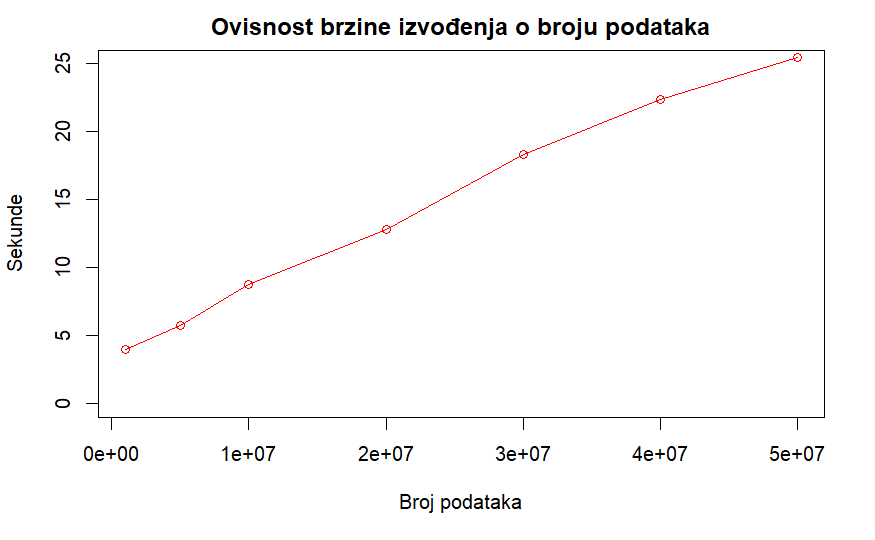
\includegraphics[width=1\linewidth]{radixPerf.png}
\caption{Figure: Prikaz performansi sekvencijalnog radix sorta}
\label{radix - performance}
\end{minipage}

Kao što prikazuju rezultati, porast vremenske složenosti je blizu linearnog. Vremenska složenost Radix sorta je \mathcal{O}(nk), gdje je \textit{n} broj podataka, a \textit{k} broj znamenki najvećeg broja.
\\
\subsection{Uvodno paralelno izvođenje}
Nakon prikaza sekvencijalnog izvođenja, napravili smo testove za "even-odd" verziju paralelnog sorta.
Rezultati testa su prikazani na slici.\\
\\
\noindent
\begin{minipage}{\linewidth}
\centering
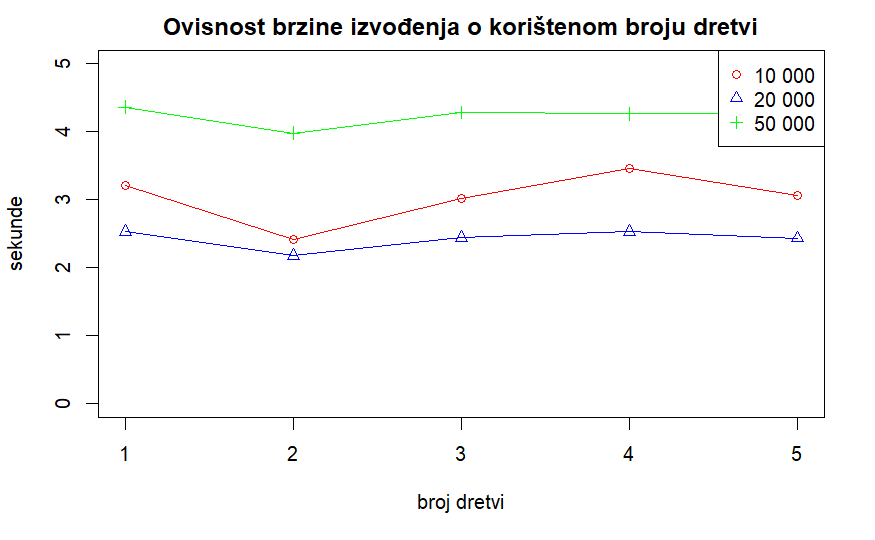
\includegraphics[width=1\linewidth]{bubblePerf.png}
\caption{Figure: Prikaz performansi bubble sorta}
\label{bubble - performance}
\end{minipage}
\\
\\


Moramo napomenuti da je za prikaz rezultata korištena logaritamska skala na y-osi, osim za rezulatate dobivene koristeći 10 000 podataka iz razloga što su vremenska izvođenja tih mjerenja bila manja od 1 sekunde te bi u logaritamskoj skali bila negativna. Rezultati su očekivani iz razloga što naša verzija implementacije paralelnog bubble sorta koristi princip podjele posla na parne i neparne pozicije liste za sortiranje. Zbog toga se jedino poboljšanje u odnosu na sekvencijalno izvođenje očituje kod korištenja 2 dretve. U tom slučaju, tako implementirani bubble sort algoritam postiže najbolje rezultate, jer jedna dretva vrši zamjenu elemenata parnih pozicija, dok druga neparnih pozicija. Zamjena elemenata vrši se po principu bubble sorta.

\subsection{Paralelno izvođenje}
Nakon razmatranja sekvencijalnog radix sorta te djelomično paralelnog bubble sorta, testirali smo sljedeće algoritme: Merge sort, Quick sort i Tim sort. Svi algoritmi se temelje na principu podijeli-pa-vladaj.
\\
\subsubsection{Merge Sort}
Merge sort je algoritam sortiranja asimptotske vremenske složenosti $O(n \log n)$. Korištenjem većeg broja dretvi, složenost se može smanjiti za konstantan broj puta. Rezultati su prikazani na slici.
\\
\noindent
\begin{minipage}{\linewidth}
\centering
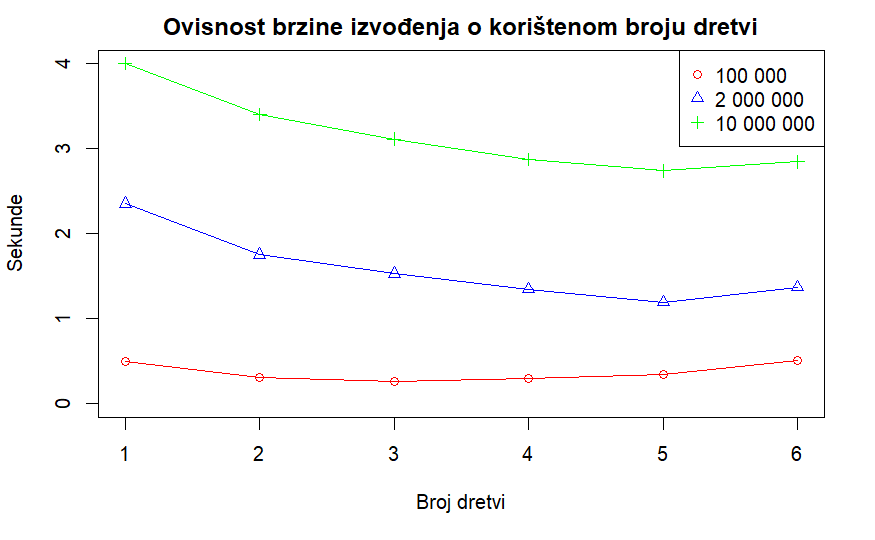
\includegraphics[width=1\linewidth]{mergePerf.png}
\caption{Figure: Prikaz performansi Merge sorta}
\label{merge - performance}
\end{minipage}

\\
Rezultati su kao i na prethodnim slikama, prikazani na logaritamskoj skali y-osi. Možemo uoćiti da na manjem broju podataka (100 000), nema poboljšanja vremena izvođenja, no iz rezultata većeg broja podataka, vidljivo je poboljšanje u odnosu na sekvencijalno izvođenje. Tijekom testiranja, pokazalo se da je optimalan broj dretvi 5. Tada je poboljšanje:
\begin{equation}
S = \frac{T_{sequential}}{T_{parallel}}
= \frac{54.9}{15.56} = 3.53
\label{eq:performance}
\end{equation}
\\
Za broj dretvi veći od 5, "overhead" mijenjanja konteksta, upravljanje većim brojem dretvi te prevelika podjela podataka na manje dijelove u našoj implementaciji utječu na degradiranje performansi. 
\\
\\

\subsubsection{Tim Sort}
Timsort je hibridni, stabilni algoritam sortiranja, izvedenica insertion sorta i merge sorta, dizajniran za dobru izvedbu na mnogim vrstama podataka. Asimptotska vremenska složenost merge sorta je $O(n \log n)$. Dobiveni rezultati prikazani su na sljedećoj slici u logaritamskoj skali na y-osi.
\\

\\

\noindent
\begin{minipage}{\linewidth}
\centering
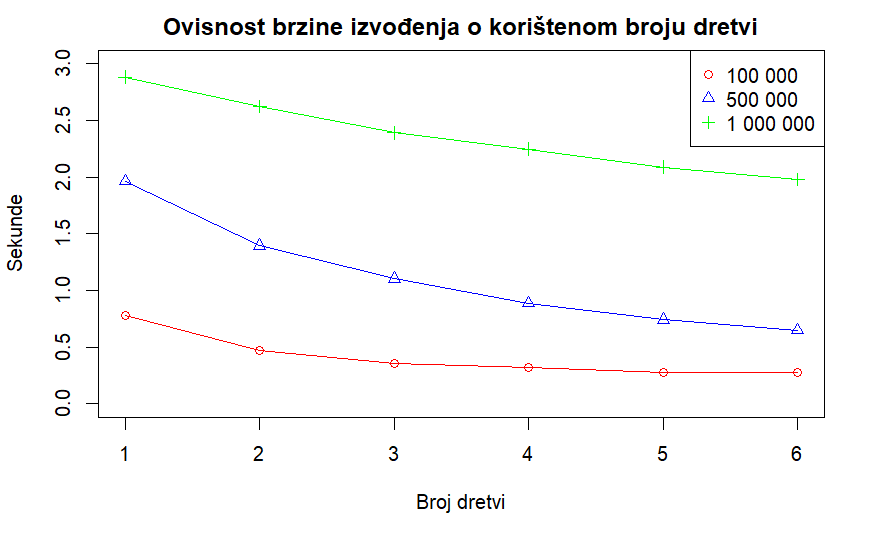
\includegraphics[width=1\linewidth]{timPerf.png}
\caption{Figure: Prikaz performansi Tim sorta}
\label{tim - performance}
\end{minipage}
\\
\\
\\

Pregledom rezultata zaključili smo da se povećanjem broja dretvi izvođenje programa ubrzava. Zbog ograničenja u hardware-u, nismo bili u mogućnosti isprobati na većem broju dretvi od 6. Poboljšanje iznosi:
\\
\begin{equation}
S = \frac{T_{sequential}}{T_{parallel}}
= \frac{17.894}{7.242} = 2.47
\label{eq:performance}
\end{equation}
\\
\\

Za razliku od Merge sorta, tim sort daje manje ubrzanje, no kao što smo napomenuli, zbog ograničenja u hardware-u, nismo bili u mogućnosti dobiti veća ubrzanja Tim sorta. Također, potrebno je napomenuti da su algoritmi testirani na različitom broju podataka te iz tog razloga usporedba nije u potpunosti definirana.
\\
\\

\subsubsection{Quick sort}
Quick sort je poslijednji algoritam sortiranja koji smo testirali. Njegova asimptotska složenost je $O(n^2)$ jer ovisi o broju pivota. Prosječna vremenska složenost iznosi $O(n \log n)$. Rezultati naših testiranja prikazani su na sljedećoj slici sa logaritamskoj skalom y-osi.
\\

\\

\noindent
\begin{minipage}{\linewidth}
\centering
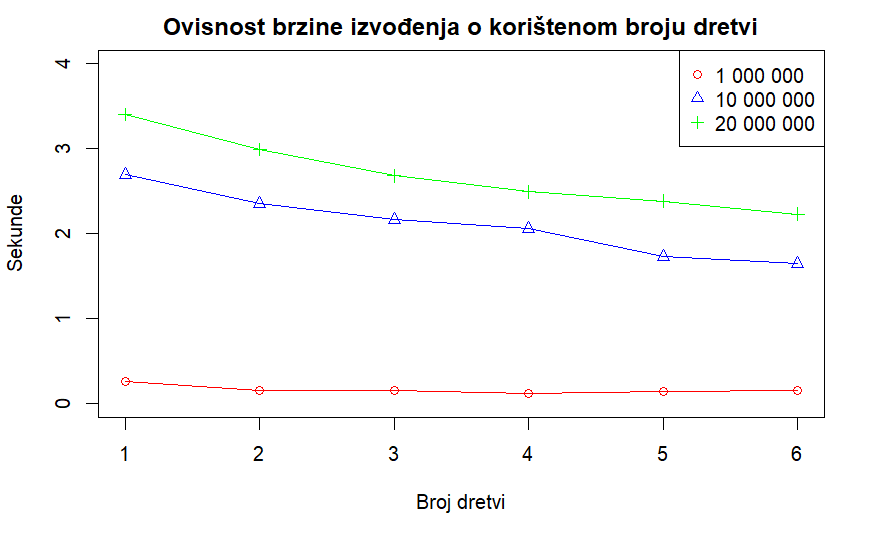
\includegraphics[width=1\linewidth]{quickPerf.png}
\caption{Figure: Prikaz performansi Quick sorta}
\label{quick - performance}
\end{minipage}
\\

\\
Kao i kod Tim sorta, nismo bili u mogućnosti vidjeti granice poboljšanja uvođenjem paralelizma, no vidimo da se povećanjem dretvi smanjuje vrijeme izvođenja.
Quick sort je pokazao relativno najbolje rezulate u izvođenju. Relativno iz razloga što nisu svi algoritmi ispitivani na jednakim brojevima podataka. Poboljšanje za 20 milijuna podataka koje smo dobili iznosi: 
\\
\begin{equation}
S = \frac{T_{sequential}}{T_{parallel}}
= \frac{30.613}{9.311} = 3.29
\label{eq:performance}
\end{equation}
\\
\\
Iz poboljšanja je također vidljivo kako je Quick sort pokazao najbolje rezultate. Merge sort je imao bolje poboljšanje, no njegovo poboljšanje nije bilo konstantno s povećanjem broja dretvi, odnosno bilo je najveće uz korištenje 5 dretvi. U procesu implementacije korištena su 2 različite metode biranja pivota, no najboljom se pokazala metoda biranja pivota između prvog, srednjeg i zadnjeg člana liste za sortiranje.

\section*{Zaključci}

Zaključno, projekt usporedbe sekvencijalnih i paralelnih algoritama za sortiranje imao je za cilj istražiti učinkovitost različitih paralelnih metoda sortiranja za velike skupove podataka.
Tijekom ovog projekta isprobali smo nekoliko različitih algoritama sortiranja. Neke nismo bili u mogućnosti paralelizirati ili smo ih djelomično paralelizirali.\\
Algoritmi s najboljim poboljšanjima u ovisnosti o broju dretvi su bili algoritmi koji se temelje na principu podijeli-pa-vladaj. \\Algoritmi za paralelno sortiranje koji koriste načelo podijeli-pa-vladaj smatraju se među najboljima jer iskorištavaju mogućnosti paralelne obrade modernih računalnih arhitektura. Oni funkcioniraju razlažući veliki problem na manje potprobleme koji se mogu samostalno riješiti, a zatim kombinirati kako bi se pronašlo rješenje izvornog problema.\\ U kontekstu našeg istraživanja, to znači da se skup podataka najprije podijeli na manje podnizove, koji se zatim paralelno neovisno sortiraju. Ovi podnizovi se zatim kombiniraju kako bi formirali konačni sortirani niz. Ovaj pristup omogućuje učinkovito korištenje više procesora ili jezgri, što može značajno smanjiti vrijeme potrebno za sortiranje velikih skupova podataka. 


\section*{Budući rad}
Buduće mogućnosti rada za projekt algoritama paralelnog sortiranja uključuju daljnju optimizaciju algoritama za paralelno sortiranje. Još uvijek ima prostora za poboljšanje u smislu učinkovitosti i performansi algoritama za paralelno sortiranje implementiranih u ovom projektu.
Također, možemo istražiti nove tehnike paralelizacije. Projekt se uglavnom usredotočio na načelo podijeli-pa-vladaj za paraleliziranje algoritama sortiranja, ali postoje i druge tehnike kao što su map-reduce ili cjevovodni paralelizam koje bi se mogle istražiti.

\\
\begin{thebibliography}{00}
\bibitem{b1} Božidar D, Dobravec T. A comparison study between sequential and parallel sorting algorithms. https://github.com/darkobozidar/sequential-vs-parallel-sort, 2015.  
\bibitem{b2} D. Zurek, M. Pietron, M. Wielgosz, and K. Wiatr, “Comparison of hybrid sorting algorithms implemented on different parallel hardware platforms,” Computer Science, vol. 14, no. 4, p. 679, 2013, issn: 2300-7036.
\bibitem{b3} K. Sujatha, P. V. N. Rao, A. A. Rao, V. G. Sastry, V. Praneeta, and R. K.
Bharat, “Multicore parallel processing concepts for effective sorting and searching,” in 2015 International Conference on Signal Processing and Communication Engineering Systems, 2015, pp. 162–166. doi: 10.1109/SPACES.2015.
7058238.
\end{thebibliography}


\end{document}
